\documentclass{article}

\usepackage[preprint]{neurips_2020}
% \usepackage[final]{neurips_2020}
% \usepackage[nonatbib]{neurips_2020}

\usepackage[utf8]{inputenc} % allow utf-8 input
\usepackage[T1]{fontenc}    % use 8-bit T1 fonts
\usepackage{hyperref}       % hyperlinks
\usepackage{url}            % simple URL typesetting
\usepackage{booktabs}       % professional-quality tables
\usepackage{amsfonts}       % blackboard math symbols
\usepackage{nicefrac}       % compact symbols for 1/2, etc.
\usepackage{microtype}      % microtypography
\usepackage{graphicx}
\usepackage{subcaption}


\title{Vector Quantized Variational Autoencoders \\on Novel Datasets}

\author{
  Shivanshu Gupta
  \And
  Kolby Nottingham
  \And
  Preethi Seshadri
}

\begin{document}

\maketitle

\begin{abstract}
    We explore using the Vector Quantized Variational Autoencoder (VQ-VAE) to generate discrete representations for the Kaokore dataset, which contains images of facial expressions from traditional Japanese illustrations (\url{https://github.com/rois-codh/kaokore}).
    The framework VQ-VAE is built on, Variational Autoencoders (VAE), learn continuous latent representations.
    While continuous representations are flexible, many real world attributes are better defined discretely, and some current state-of-the art model architectures, like transformers, only work with discrete data. Additionally, VAEs have been shown to exhibit posterior collapse, which means that latent codes are ignored. 
    In this project, we experiment with VQ-VAEs on a novel dataset and design experiments to test the advantages and disadvantages of multiple VQ-VAE variations.
    %Since the VQ-VAE paper uses CIFAR10 and 128x128 ImageNet images, there might be additional experimentation and training required to achieve good performance on the Kaokore dataset.
    % VQ-VAEs have been paired with the transformer architecture which, while scalable, can require a lot of compute, so we will experiment with making the method more compute efficient.  % Not sure what to put in this sentence??? Maybe something generic for now.
    Our results indicate that while the original VQ-VAE algorithm learns faster than some of its successors, it does not achieve the same level of performance. 
\end{abstract}

\section{Introduction}

Generative machine learning models learn a distribution $p(x,y)$ for data instances $x$ and labels $y$. Compared to discriminative machine learning models that learn $p(y|x)$, generative models can be more difficult to learn but come with added benefits. One use case for generative machine learning models is mapping data instances to a latent space. Once mapped to a latent space, latent variables can be used as a compressed representation of a data instances or to sample and generate new data instances.

One generative machine learning model that learns latent variable representations of data is the variational autoencoder (VAE). VAEs learn a latent variable representation of each datapoint with an encoder module. Simultanously, a decoder module learns to reconstruct the original image from the latent variables.

Traditional VAEs learn a latent space that is associated with a probablility distribution of continuous variables. Vector quantized variational autoencoders (VQ-VAE) learn discrete latent variables instead. Discrete variables are cometimes advantageous because real world data can often be summarized by categorical features. 

In this work, we compare two variations of VQ-VAEs. The second variation (VQ-VAE2) was released as a follow up to VQ-VAEs and introduces a hierarchical structure for the model. We go into further detail comparing the algorithms in section \ref{vqvae}. We implement each of these methods and run experiemnts with each on the Kaokore dataset. To the best of our knowledge, this is the first time VAEs have been used to learn a latent space for this dataset.

\section{Background}

Generative models...

Autoencoders...

\section{Vector Quantized Variational Autoencoders} \label{vqvae}

\subsection{VAE}
\subsection{VQ-VAE}
\subsection{VQ-VAE2}

\section{Experiments}

In a series of experiments, we compare traditional VAEs to VQ-VAEs. We first...

\subsection{Kaokore Dataset}

The Kaokore dataset consists of...

\subsection{Results}

\begin{table}
    \centering
    \begin{tabular}{c c c}
        & Commitment Loss & Reconstruction Loss \\
        \hline
        VQ-VAE & 0.0793 (0.0027) & 0.0056 (0.0001) \\
        VQ-VAE2 & 0.0025 (0.0035) & 0.0005 (0.0008)
    \end{tabular}
    \caption{Commitment loss and reconstruction loss on the Kaokore testset for both algorithms.}
\end{table}

\begin{figure}
    \centering
    \begin{subfigure}{.49\linewidth}
        \centering
        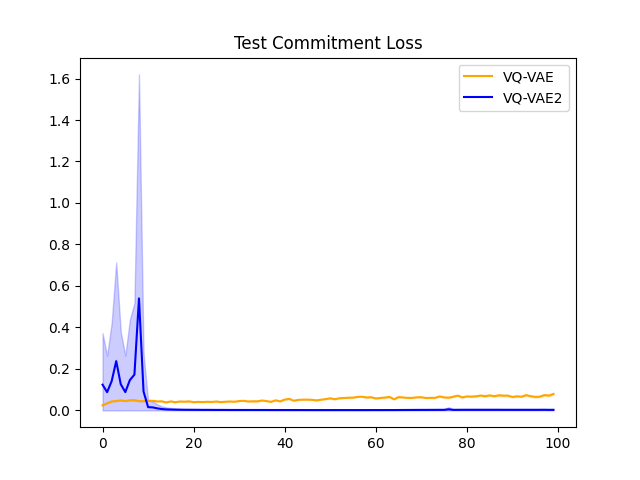
\includegraphics[width=\linewidth]{commit.png}
        \caption{Commitment loss over 100 epochs.}
    \end{subfigure}
    \begin{subfigure}{.49\linewidth}
        \centering
        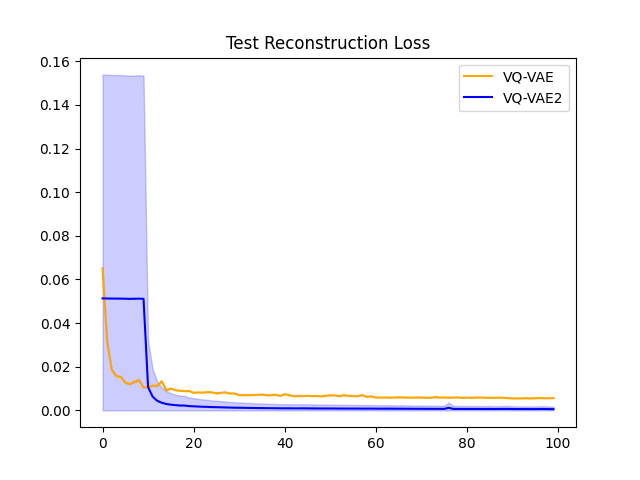
\includegraphics[width=\linewidth]{recon.png}
        \caption{Reconstruction loss over 100 epochs.}
    \end{subfigure}
\end{figure}

\begin{figure}
    \centering
    \includegraphics[width=\linewidth]{samples.png}
    \caption{The first six rows of images show samples at 1, 12, 14, 16, 18, and 100 epochs for VQ-VAE (left) and VQ-VAE2 (right). The final row shows the cooresponding images from the testset.}
\end{figure}

As indicated in table...

\section{Conclusion}

The authors of the VQ-VAE paper presented promising results. However, bsaed on our experiments, we conclude that it is not strictly better than VAE on every dataset...

\end{document}